\documentclass[]{article}

% Imports the catppuccin theme, using the mocha flavor,
% from the directory above. Actual implementation
% wouldn't need the import package unless the theme
% and the document are in different directories.
\usepackage{import}
\usepackage{xcolor}
% \usepackage{fancyhdr}
\usepackage{cancel}
\usepackage{mathtools}

% For permutations and combinations
\newcommand\Myperm[2][^n]{\prescript{#1\mkern-2.5mu}{}P_{#2}}
\newcommand\Mycomb[2]{\prescript{#1\mkern-0.5mu}{}C_{#2}}

% Colors
\definecolor{yorhabg}{HTML}{FFFFFF}
\definecolor{yorhafg}{HTML}{000000}
\definecolor{yorhagrid}{HTML}{B5AF9C}
\definecolor{mred}{HTML}{D67069}
\definecolor{mblue}{HTML}{6887A1}

\pagecolor{yorhabg}
\color{yorhafg}

\usepackage{preamble}

% Removes padding above title
\usepackage{titling}
\setlength{\droptitle}{-10em}

% Font package
\usepackage[T1]{fontenc}

\usepackage{fouriernc}

\usepackage{sectsty}
\usepackage{graphicx}
\usepackage{amsmath}
\usepackage{amsfonts}
\usepackage{amssymb}
\usepackage[skins, most]{tcolorbox}
\usepackage{enumitem}

\DeclareMathOperator{\sgn}{sgn}

\usepackage{tikz}
\usepackage{eso-pic}
\usetikzlibrary{calc,shadows.blur}
\usetikzlibrary{angles, quotes}
\usetikzlibrary{3d}

% Margins
\topmargin=0in
\evensidemargin=0in
\oddsidemargin=0in
\textwidth=6.5in
\textheight=9.0in
\headsep=0.25in

\AtBeginEnvironment{tcolorbox}{\small}

\newtcolorbox{imp}{enhanced,arc=0mm,colback=yorhabg,colframe=mred,leftrule=10mm,coltext=yorhafg,%
overlay={\node[anchor=west,outer sep=2pt] at (frame.west) {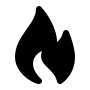
\includegraphics[width=6mm]{images/imageb.png}}; }}

\newtcolorbox{shortcut}{enhanced,arc=0mm,colback=yorhabg,colframe=mred,leftrule=10mm,coltext=yorhafg, coltitle=yorhabg, title=\texttt{Shortcut.}, 
overlay={\node[anchor=west,outer sep=2pt] at (frame.west) {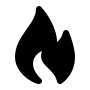
\includegraphics[width=6mm]{images/imageb.png}}; }}

\newtcolorbox{question}[1]{
    enhanced, 
    colback=yorhabg,
    colframe=mblue,
    coltext=yorhafg,
    coltitle=yorhabg,
    attach boxed title to top left={yshift*=-\tcboxedtitleheight}, 
    title=\texttt{#1},
    boxed title size=title,
    boxed title style={%
        rounded corners=northeast, 
        rounded corners=northwest, 
        colback=tcbcolframe, 
        boxrule=0pt,
    },
    underlay boxed title={%
        \path[fill=tcbcolframe] (title.south west)--(title.south east) 
            to[out=0, in=180] ([xshift=5mm]title.east)--
            (title.center-|frame.east)
            [rounded corners=5pt] |- 
            (frame.north) -| cycle; 
    },
}
% \pagestyle{fancy}
% \fancyhf{}  % Clear all default header/footer
% \fancyhead[L]{\small Satyajit Datta \\ 1012033336}  % Top-left, small font
\newcommand\bb[1]{\textcolor{yorhafg}{\textbf{#1}}}

\title{\textbf{CSCA67 - Exercises \#4}}
\author{Satyajit Datta \\ 1012033336}
\date{\today}

\begin{document}

\maketitle

\begin{question}{2}
Translate the specifications below into English. Let $F(p)$ be “printer $p$ is out of service”, $B(p)$
be “printer $p$ is busy”, $L(j)$ be “print job $j$ is lost”, and $Q(j)$ be is “print job $j$ is queued”.
Universe of discourse for $F$ and $B$ is printers, and universe of discourse for $L$ and $Q$ is print
jobs.

\begin{enumerate}[label=\textbf{\arabic*.}]
    \item $(\exists p, (F(p) \land B(p))) \rightarrow (\exists j, L(j))$
    \item $(\forall p, B(p)) \rightarrow (\exists j, Q(j))$
    \item $(\exists j, (Q(j) \land L(j))) \rightarrow (\exists p, F(p))$
    \item $((\forall p, B(p)) \land (\forall j, Q(j))) \rightarrow (\exists j, L(j))$
\end{enumerate}
\end{question}

\begin{enumerate}[label=\textbf{\arabic*.}]
    \item If there exists a printer that is both out of service and busy, then there exists a print job that is lost.
    \item If all printers are busy, then at least one print job is queued.
    \item If there exists a print job that is both queued and lost, then there is a printer that is out of service.
    \item If all printers are busy and all jobs are queued, then there is a job that is lost.
\end{enumerate}

\begin{question}{3}
   Translate each of these statements into logical expressions using predicates, quantifiers, and
logical connectives. 

\begin{enumerate}[label=\textbf{\arabic*.}]
    \item Something is not in the correct place.
    \item All tools are in the correct place and are in excellent condition.
    \item Everything is in the correct place and in excellent condition.
    \item Nothing is in the correct place and in excellent condition.
    \item At least one of your tools is not in the correct place, but it is in excellent condition.
\end{enumerate}
\end{question}

Let the universe of discourse be things. Let the set $T$ be the set of all tools. Let $E(x)$ be "$x$ is in excellent condition."
Let $P(x)$ be "$x$ is in the correct place".

\begin{enumerate}[label=\textbf{\arabic*.}]
    \item $\exists x, \neg P(x)$
    \item $\forall x \in T, P(x) \land E(x)$
    \item $\forall x, P(x) \land E(x)$
    \item $\forall x, \neg(P(x) \land E(x))$
    \item $\exists x \in T, \neg P(x) \land E(x)$
\end{enumerate}

\section*{Negation.}

Analyse the logical forms of the following statements (where applicable). Negate each statement,
and then re-express the results as equivalent positive statements.

\begin{question}{1}
    There is someone in this class who does not have a roommate. Let $C(x)$ be “$x$ is in this class”,
    $R(x)$ be “$x$ has a roommate”. Universe of discourse is people.
\end{question}

The logical form of this statement is:

\begin{center}
    $\exists x, C(x) \land \neg R(x)$
\end{center}

Negation of this statement is:

\begin{align*}
    & \neg(\exists x, C(x) \land \neg R(x)) \\
    \Rightarrow & \forall x, \neg(C(x) \land \neg R(x)) \\
    \Rightarrow & \forall x, \neg C(x) \lor \neg\neg R(x) \\
    \Rightarrow & \forall x, \neg C(x) \lor R(x) \\
    \Rightarrow & \forall x, C(x) \rightarrow R(x)
\end{align*}

The English version of this statement would be:

\begin{center}
    \bf{Everybody that is in this class has a roommate.}
\end{center}

\begin{question}{2}
    There is someone in this class who does not have a roommate. Let $C(x)$ be “$x$ is in this class”,
$R(x, y)$ be “$x$ and $y$ are roommates”. Universe of discourse is people.
\end{question}

The logical form of this statement is:

\begin{center}
    $\exists x, (C(x) \land \forall y, \neg R(x, y))$
\end{center}

Negation of this statement would be

\begin{align*}
    &  \neg(\exists x, (C(x) \land \forall y, \neg R(x, y))) \\
    \Rightarrow &  \forall x, \neg (C(x) \land \forall y, \neg R(x, y)) \\
    \Rightarrow &  \forall x, \neg C(x) \lor \neg(\forall y, \neg R(x, y)) \\
    \Rightarrow &  \forall x, \neg C(x) \lor (\exists y, \neg\neg R(x, y)) \\
    \Rightarrow &  \forall x, \neg C(x) \lor (\exists y, R(x, y)) \\
    \Rightarrow & \forall x, C(x) \rightarrow  (\exists y, (R(x, y)))
\end{align*}

The English version of this statement would be:

\begin{center}
    \bf{If someone is in this class, then they have a roommate.}
\end{center}

\begin{question}{3}
    Everyone likes someone, but no one likes everyone. Let $L(x, y)$ be “$x$ likes $y$”. Universe of
discourse is people.
\end{question}

The logical form of this statement is:

\begin{center}
    $\forall x, \exists y, L(x, y) \land \neg \exists x, \forall y, L(x, y)$
\end{center}

Negation of this statement would be

\begin{align*}
    & \neg((\forall x, \exists y, L(x, y) \land \neg (\exists x, \forall y, L(x, y)))) \\
    \Rightarrow & \neg (\forall x, \exists y, L(x, y)) \lor \neg\neg(\exists x, \forall y, L(x, y)) \\
    \Rightarrow & (\exists x, \forall y, \neg L(x, y)) \lor (\exists x, \forall y, L(x, y)) \\
\end{align*}

The English version of this statement would be:

\begin{center}
    \bf{Either someone doesn't like anyone, or there is someone that likes everyone.}
\end{center}


\begin{question}{4}
    $\forall a \in A, \exists b \in B, (a \in C \leftrightarrow b \in C).$ Universe of discourse is set $U$.
\end{question}

Negation of this statement would be

\begin{align*}
\neg \Big( \forall a \in A, \exists b \in B, \ (a \in C \leftrightarrow b \in C) \Big) 
&= \exists a \in A, \forall b \in B, \ \neg (a \in C \leftrightarrow b \in C) \\[2mm]
&= \exists a \in A, \forall b \in B, \ \neg \big( (a \in C \rightarrow b \in C) \land (b \in C \rightarrow a \in C) \big) \\[1mm]
&= \exists a \in A, \forall b \in B, \ \neg \big( (\neg(a \in C) \lor b \in C) \land (\neg(b \in C) \lor a \in C) \big) \\[1mm]
&= \exists a \in A, \forall b \in B, \ \big( \neg(\neg(a \in C) \lor b \in C) \lor \neg(\neg(b \in C) \lor a \in C) \big) \\[1mm]
&= \exists a \in A, \forall b \in B, \ \big( (a \in C \land b \notin C) \lor (b \in C \land a \notin C) \big)
\end{align*}

\begin{question}{5}
    $\forall y, y>0 \rightarrow (\exists x, ax^2 + bx + c = y)$. Universe of discourse is $\mathbb{R}$.
\end{question}

Negation of this statement would be

\begin{align*}
    \neg(\forall y, y>0 \rightarrow (\exists x, ax^2 + bx + c = y)) \\
    \exists y, \neg(y>0 \rightarrow (\exists x, ax^2 + bx + c = y)) \\
    \exists y, \neg(\neg(y>0) \lor (\exists x, ax^2 + bx + c = y)) \\
    \exists y, \neg\neg(y>0) \land \neg(\exists x, ax^2 + bx + c = y) \\
    \exists y, y>0 \land (\forall x, \neg(ax^2 + bx + c = y)) \\
    \exists y, y>0 \land (\forall x, (ax^2 + bx + c \ne y)) \\
\end{align*}

\end{document}$